\section{QA evidence: executed scope and limits}
\label{sec:qa-evidence}

\subsection{Evidence boundary}

This section reports only evidence present in the repository and the dated QA
report. A designed scenario is not an executed scenario. The current record
covers a real local Selenium run, its TestLink read-back, and infrastructure
checks; it does not certify the complete product regression.

\begin{center}
\begin{tabular}{lll}
\toprule
\textbf{Document ID} & \textbf{Observed action} & \textbf{Recorded result}\\
\midrule
\Code{COMAL-QA-001} & Selenium enters \Code{42} in the operator view and the public view reads \Code{42}. & \textcolor{comalgreen}{PASS}\\
\Code{COMAL-QA-003} & Selenium submits an invalid capture and verifies that state is not mutated. & \textcolor{comalgreen}{PASS}\\
\Code{COMAL-QA-011} & Selenium corrects the last capture without announcing it. & \textcolor{comalgreen}{PASS}\\
\Code{INFRA-ADAPTER-001} & Deliberate negative report is written and read back as TestLink status \Code{f}. & \textcolor{comalgreen}{PASS (control)}\\
\bottomrule
\end{tabular}
\end{center}

\Evidence{qa/management/reporte-final.md; qa/management/alcance-y-entregable-final.md}

The integration report identifies TestLink case \Code{COMAL-50}, build
\Code{7}, execution \Code{9}, and the negative control in execution
\Code{10}. The latest UI suite created build \Code{13} and read back
executions \Code{21}, \Code{22}, and \Code{23} as PASS. These identifiers are
the observed mappings for those runs; they are not interchangeable with the
documentary \Code{COMAL-QA-xxx} identifiers.

\subsection{TestLink and Docker infrastructure}

The local TestLink stack is defined in \Code{qa/testlink/compose.yaml}. It
binds the web service to \Code{127.0.0.1:8090}, uses pinned image digests, and
persists the database, application, logs, and upload areas in named volumes.
The repository records successful checks for login, authenticated index,
XML-RPC, and HTTP blocking of \Code{/install} and \Code{/docs}. Recreating
containers without removing volumes preserved the schema, catalog, executions,
and attachment record.

\begin{center}
\begin{tabular}{ll}
\toprule
\textbf{Component} & \textbf{Repository evidence}\\
\midrule
TestLink & \Code{qa/testlink/setup.ps1}, \Code{verify.ps1}, XML-RPC adapter, local-only endpoint\\
Catalog & 43 designed scenarios in \Code{qa/catalogo/casos-prueba.json}; 12 use cases and traceability documentation\\
Persistence & MySQL and TestLink named volumes; persistence check recorded as PASS\\
Automation & \Code{qa:integration} and \Code{qa:ui}; UI report targets the three COMAL cases above\\
\bottomrule
\end{tabular}
\end{center}

\subsection{Designed coverage versus executed coverage}

The catalog contains 43 scenarios. Three product scenarios were actually
executed by the reported UI suite. The remaining 40 are still
\textcolor{comalamber}{planned}; this document deliberately does not describe
them as passed or executed. The catalog import also states that importing
cases creates no executions.

\subsection{Attachments and local screenshots}

The UI run preserved screenshots locally under
\Code{test-results/qa-ui/evidence/} according to the QA report. The same report
records that TestLink returned the attachment insertion error \Code{6002} for
the three UI attachments. Consequently, this document does not claim that
those files are remote TestLink attachments: the result and notes are
auditable in TestLink, while the screenshots remain local evidence. The three execution screenshots were
promoted to the documentation artifact directory so that this report remains
reproducible outside the ignored \Code{test-results} directory:

\begin{center}
\IfFileExists{qa/evidence/COMAL-QA-001-publica-42.jpg}{%
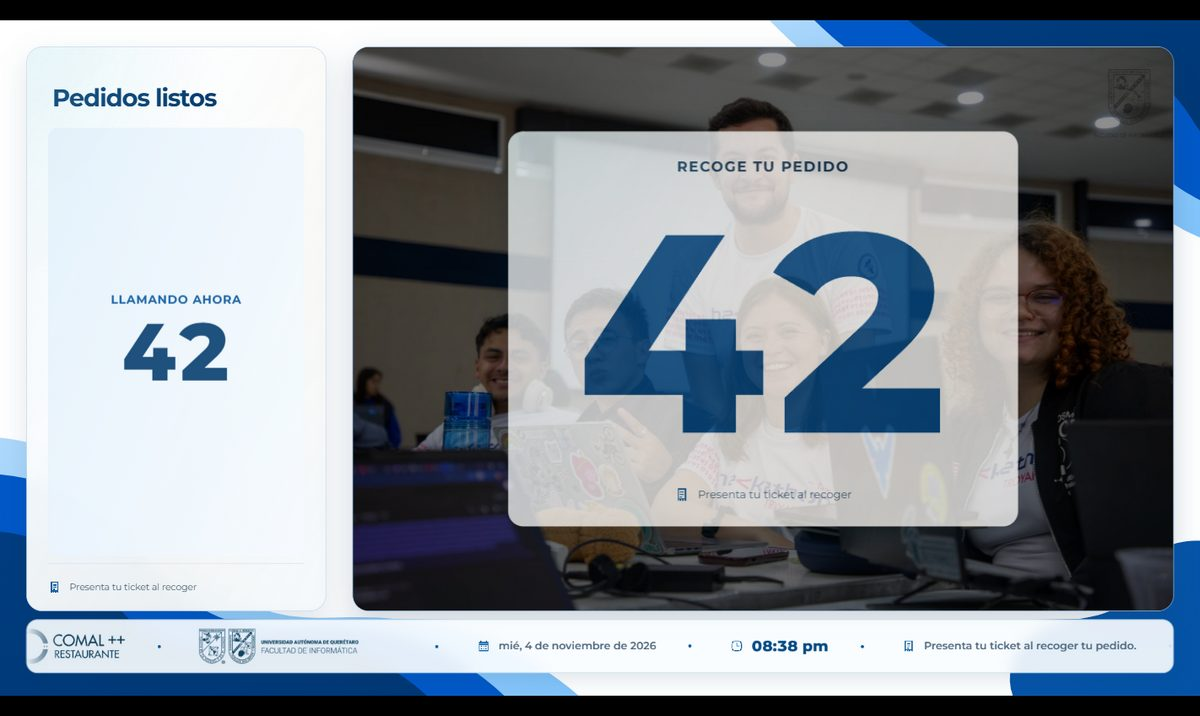
\includegraphics[width=.47\textwidth]{qa/evidence/COMAL-QA-001-publica-42.jpg}\hfill
}{}
\IfFileExists{qa/evidence/COMAL-QA-003-invalid-capture.jpg}{%
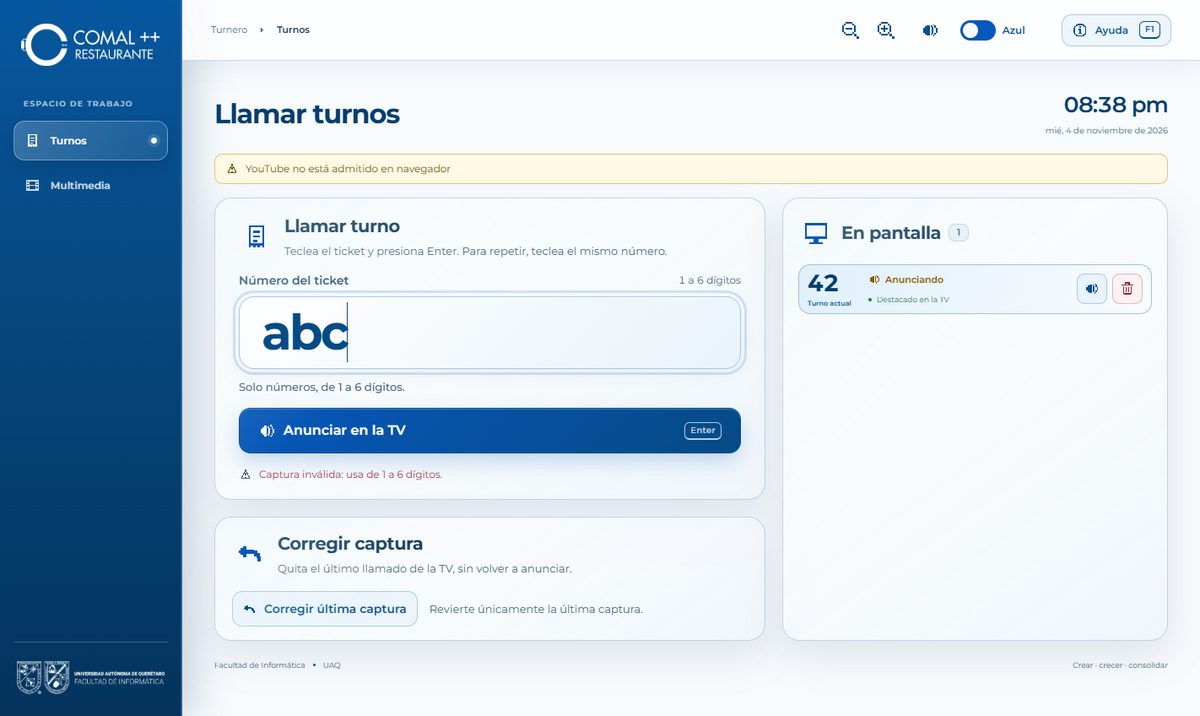
\includegraphics[width=.47\textwidth]{qa/evidence/COMAL-QA-003-invalid-capture.jpg}
}{}
\end{center}
\emph{Execution evidence for \Code{COMAL-QA-001} and \Code{COMAL-QA-003}.}

\begin{center}
\IfFileExists{qa/evidence/COMAL-QA-011-correct-last-capture.jpg}{%
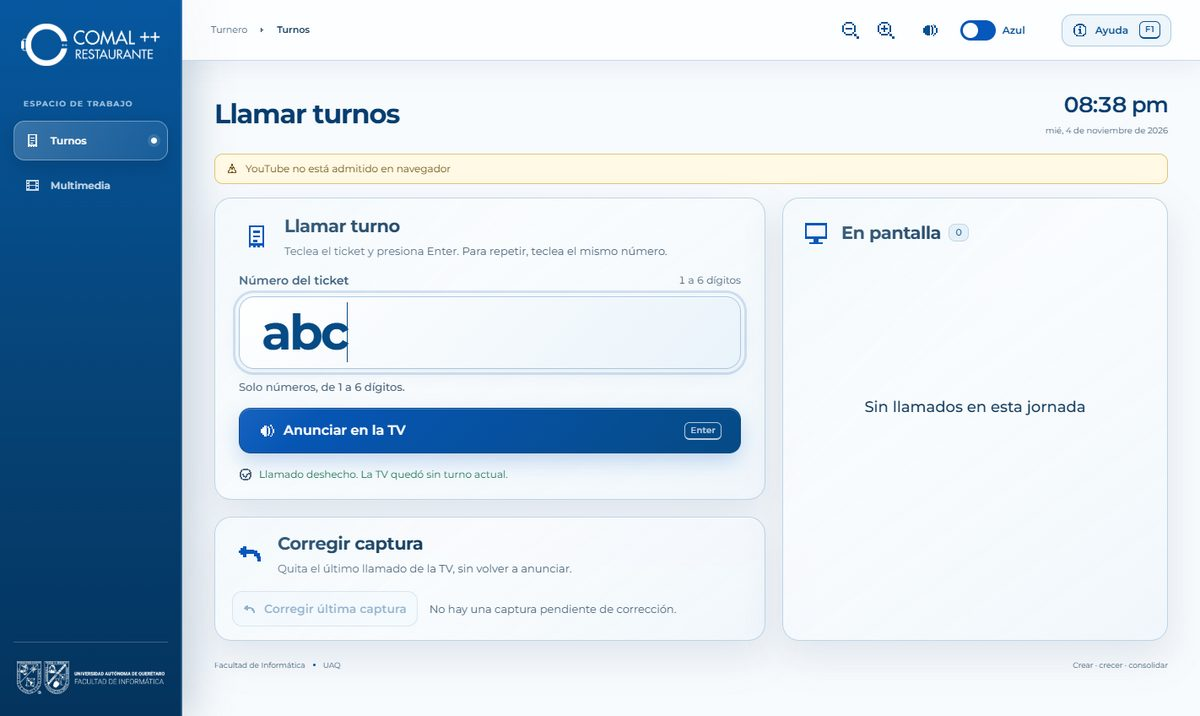
\includegraphics[width=.47\textwidth]{qa/evidence/COMAL-QA-011-correct-last-capture.jpg}
}{}
\end{center}
\emph{Execution evidence for \Code{COMAL-QA-011}.}

\subsection{Pending validation and limitations}

\begin{itemize}
\item Execute and analyze the remaining 40 catalog scenarios; no result is
  inferred from their design or import.
\item Repeat the UI attachment flow after resolving or documenting TestLink
  error \Code{6002}; retain the local copies and upload notes meanwhile.
\item Validate physical audio, TV/monitor legibility, prolonged jornada
  performance, Windows installation/startup, and signing on target hardware.
\item Keep the TestLink image and PHP 7.4 compatibility limitation under
  review; the repository does not claim current upstream support.
\end{itemize}

\subsection{Reproducible commands}

From the repository root, the evidence documents the following PowerShell
workflow. Credentials remain in the ignored local \Code{qa/testlink/.env}.

\begin{CodeBlock}
.\qa\testlink\setup.ps1
.\qa\testlink\verify.ps1
npm run qa:integration
npm run qa:ui
node qa\automation\import-catalog.mjs
\end{CodeBlock}

The commands above are a reproduction procedure, not a claim that every
command was rerun while composing this document.
